\documentclass[tikz,border=6pt]{standalone}
\usepackage[T1]{fontenc}
\usepackage{lmodern}
\usepackage{amsmath}
\usepackage{pgfplots}
\pgfplotsset{compat=1.18}
\usetikzlibrary{arrows.meta,positioning,fit,backgrounds,shapes.geometric,calc}
\definecolor{navy}{HTML}{16324F}
\definecolor{tealC}{HTML}{007F82}
\definecolor{amberC}{HTML}{D97706}
\definecolor{coralC}{HTML}{C2410C}
\definecolor{redC}{HTML}{DC2626}
\definecolor{mintC}{HTML}{059669}
\definecolor{slateC}{HTML}{64748B}
\definecolor{paleBg}{HTML}{F4F7FA}
\definecolor{softTeal}{HTML}{E6F4F4}
\definecolor{softNavy}{HTML}{EAF0F6}
\definecolor{softAmber}{HTML}{FEF3C7}
\begin{document}

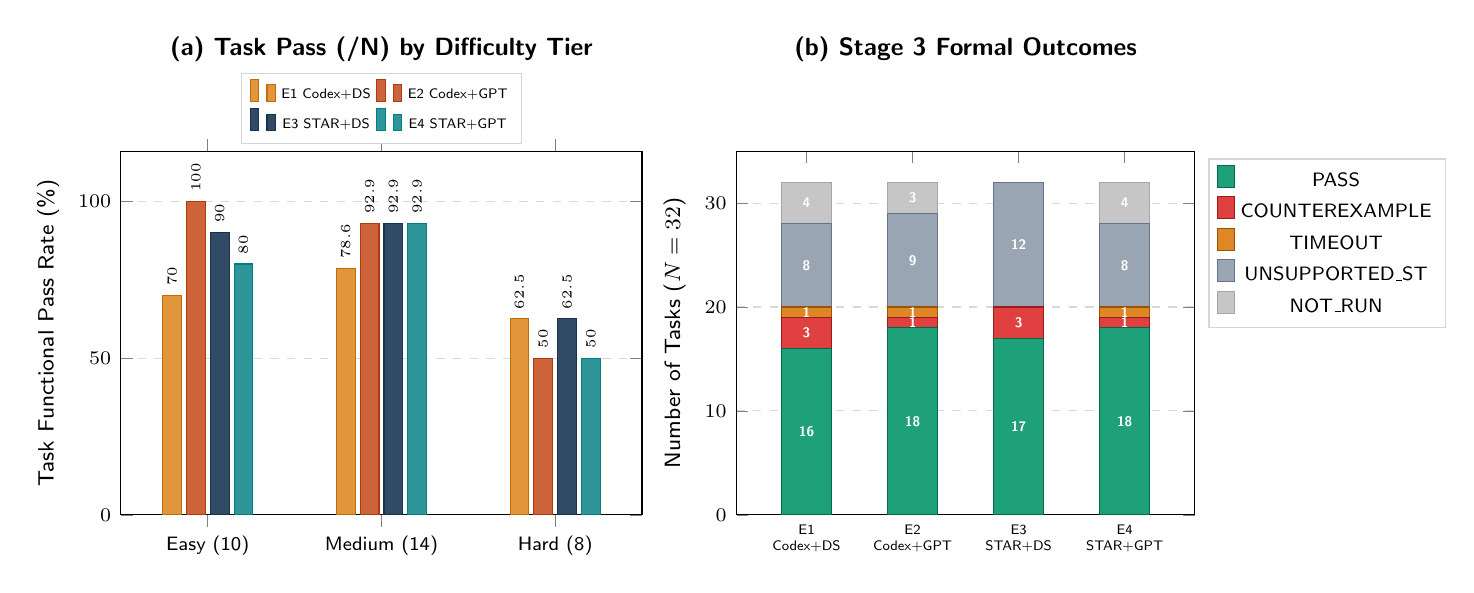
\begin{tikzpicture}
\begin{axis}[
    name=leftax,
    ybar=1.8pt,
    bar width=6.8pt,
    width=8.2cm,
    height=6.2cm,
    ymin=0, ymax=116,
    ylabel={\footnotesize Task Functional Pass Rate (\%)},
    xtick={0,1,2},
    xticklabels={Easy (10),Medium (14),Hard (8)},
    tick label style={font=\scriptsize\sffamily},
    label style={font=\footnotesize\sffamily},
    title={\small\sffamily\bfseries (a) Task Pass (/N) by Difficulty Tier},
    title style={yshift=8mm},
    legend style={at={(0.5,1.02)}, anchor=south, legend columns=2, font=\tiny\sffamily, draw=navy!20, fill=white},
    nodes near coords,
    every node near coord/.append style={font=\tiny\sffamily, rotate=90, anchor=west},
    ymajorgrids=true,
    grid style={dashed, gray!30},
    enlarge x limits=0.25,
]
\addplot[fill=amberC!78, draw=amberC!90!black] coordinates {(0,70.0) (1,78.6) (2,62.5)};
\addplot[fill=coralC!82, draw=coralC!90!black] coordinates {(0,100.0) (1,92.9) (2,50.0)};
\addplot[fill=navy!88, draw=navy] coordinates {(0,90.0) (1,92.9) (2,62.5)};
\addplot[fill=tealC!82, draw=tealC] coordinates {(0,80.0) (1,92.9) (2,50.0)};
\legend{E1 Codex+DS, E2 Codex+GPT, E3 STAR+DS, E4 STAR+GPT}
\end{axis}

\begin{axis}[
    at={($(leftax.south east)+(12mm,0)$)},
    anchor=south west,
    ybar stacked,
    bar width=18pt,
    width=7.4cm,
    height=6.2cm,
    ymin=0, ymax=35,
    ylabel={\footnotesize Number of Tasks ($N=32$)},
    xtick={0,1,2,3},
    xticklabels={E1\\Codex+DS, E2\\Codex+GPT, E3\\STAR+DS, E4\\STAR+GPT},
    x tick label style={font=\tiny\sffamily, align=center},
    tick label style={font=\scriptsize\sffamily},
    label style={font=\footnotesize\sffamily},
    title={\small\sffamily\bfseries (b) Stage 3 Formal Outcomes},
    title style={yshift=8mm},
    legend style={at={(1.03,0.98)}, anchor=north west, font=\scriptsize\sffamily, draw=navy!20, fill=white},
    nodes near coords={\pgfmathfloattoint{\pgfplotspointmeta}\ifnum\pgfmathresult>0 \pgfmathresult\fi},
    every node near coord/.append style={font=\tiny\sffamily\bfseries, color=white, inner sep=0pt},
    ymajorgrids=true,
    grid style={dashed, gray!30},
    enlarge x limits=0.22,
]
\addplot[fill=mintC!90, draw=mintC!70!black] coordinates {(0,16) (1,18) (2,17) (3,18)};
\addplot[fill=redC!88, draw=redC!70!black] coordinates {(0,3) (1,1) (2,3) (3,1)};
\addplot[fill=amberC!88, draw=amberC!70!black] coordinates {(0,1) (1,1) (2,0) (3,1)};
\addplot[fill=slateC!65, draw=slateC] coordinates {(0,8) (1,9) (2,12) (3,8)};
\addplot[fill=gray!45, draw=gray!70] coordinates {(0,4) (1,3) (2,0) (3,4)};
\legend{PASS, COUNTEREXAMPLE, TIMEOUT, UNSUPPORTED\_ST, NOT\_RUN}
\end{axis}
\end{tikzpicture}
\end{document}
